\documentclass[12pt]{article}

% Language setting
% Replace `english' with e.g. `spanish' to change the document language
\usepackage[polish]{babel}
\usepackage{polski}
\usepackage{mathtools}
% Set page size and margins
% Replace `letterpaper' with `a4paper' for UK/EU standard size
\usepackage[letterpaper,top=2cm,bottom=2cm,left=2cm,right=2cm, marginparwidth=1.75cm]{geometry}
\usepackage{extarrows}
\usepackage{multicol}
\usepackage{amsmath}
\usepackage{graphicx}
\usepackage[hidelinks]{hyperref}
\usepackage{listings}
\usepackage{physics}
\usepackage{color} %red, green, blue, yellow, cyan, magenta, black, white
\definecolor{mygreen}{RGB}{28,172,0} % color values Red, Green, Blue
\definecolor{mylilas}{RGB}{170,55,241}
\lstset{language=Matlab,%
    %basicstyle=\color{red},
    breaklines=true,%
    morekeywords={matlab2tikz},
    keywordstyle=\color{blue},%
    morekeywords=[2]{1}, keywordstyle=[2]{\color{black}},
    identifierstyle=\color{black},%
    stringstyle=\color{mylilas},
    commentstyle=\color{mygreen},%
    showstringspaces=false,%without this there will be a symbol in the places where there is a space
    numbers=left,%
    numberstyle={\tiny \color{black}},% size of the numbers
    numbersep=9pt, % this defines how far the numbers are from the text
    emph=[1]{for,end,break},emphstyle=[1]\color{red}, %some words to emphasise
    %emph=[2]{word1,word2}, emphstyle=[2]{style},    
    extendedchars=true,
    literate={ą}{{\k a}}1
  		     {Ą}{{\k A}}1
           {ż}{{\. z}}1
           {Ż}{{\. Z}}1
           {ź}{{\' z}}1
           {Ź}{{\' Z}}1
           {ć}{{\' c}}1
           {Ć}{{\' C}}1
           {ę}{{\k e}}1
           {Ę}{{\k E}}1
           {ó}{{\' o}}1
           {Ó}{{\' O}}1
           {ń}{{\' n}}1
           {Ń}{{\' N}}1
           {ś}{{\' s}}1
           {Ś}{{\' S}}1
           {ł}{{\l}}1
           {Ł}{{\L}}1
}

\begin{document}
\begin{titlepage}
       \begin{center}
       \vspace*{1cm}
       
       \textbf{Projekt 2}   
       
       \vspace{1.5cm}
       
       \textbf{Marcin Skrzypczak} \\
        Modelowanie Matematyczne \\
        Prowadzący: dr inż. Jakub Wagner
        
       \vfill       
       
       Politechnika Warszawska\\       
       Wydział Matematyki i Nauk Informacyjnych\\
       Warszawa \\
       30.01.2022 \\
       
       \vspace{1.5cm}

   \end{center}
          Oświadczam, że niniejsza praca, stanowiąca podstawę do uznania osiągnięcia efektów uczenia się z przedmiotu  Modelowanie matematyczne, została wykonana przeze mnie samodzielnie. \\
          Marcin Skrzypczak, 320735
\end{titlepage}

\tableofcontents
\break

\section{Sformułowanie zadania}
    Równania Lotki-Volterry służą do modelowania liczebności populacji dwóch gatunków, między którymi występuje zależność drapieżnik-ofiara:
    \begin{flalign}
        & \quad  \dv{x}{t}(t)=r_xx(t)+r_{xy}x(t)y(t)+r_{xx}x^2(t) &
    \end{flalign}
    \begin{flalign}
        & \quad  \dv{y}{t}(t)=r_yy(t)+r_{yx}x(t)y(t)+r_{yy}y^2(t) &
    \end{flalign}
    gdzie $x$ to liczebność populacji gatunku ofiary, $y$ - liczebność populacji gatunku drapieżnika, $t$ - czas, $r_x,r_y,x_{xy},r_{yx},r_{xx},r_{yy}\in R$ - parametry modelu, $t_1,\dots,t_N$ - chwile, w których dokonano pomiaru oraz $\tilde{x}_1,\dots,\tilde{x}_N$ i $\tilde{y}_1,\dots,\tilde{y}_N$ wyniki pomiaru.
    Zadanie skupia się na numerycznym przybliżeniu parametrów modelu opisującego zadane dane. Obliczenia zostały przeprowadzone przy użyciu następujących metod rozwiązywania RRZ:
    \begin{enumerate}
        \item jawnej metody Eulera:
        \begin{flalign*}
            & \quad \hat{x}_n=\hat{x}_{n-1}+f(t_{n-1},\hat{x}_{n-1})\Delta t &
        \end{flalign*}
        \item jawnej metody Adamsa-Bashfortha trzeciego rzędu:
        \begin{flalign*}
            & \quad \hat{x}_n=\hat{x}_{n-1}+\frac{1}{12}\left[23f(t_{n-1},\hat{x}_{n-1})-16f(t_{n-2},\hat{x}_{n-2})+5f(t_{n-3},\hat{x}_{n-3})\right]\Delta t &
        \end{flalign*}
        \item niejawnej metody Eulera
        \begin{flalign*}
            & \quad \hat{x}_n=\hat{x}_{n-1}+f(t_{n},\hat{x}_{n})\Delta t &
        \end{flalign*}
    \end{enumerate}
    
\section{Modelowanie populacji ofiar}
    Początkowym celem będzie wyznaczenie wartości $r_x,r_{xy}$ i $r_{xx}$ minimalizujących wskaźnik dopasowania modelu do danych, określonego wzorem
    \begin{flalign*}
        &\quad J_x\equiv\sum\limits^{N}_{n=2}(\hat{x}_n-\tilde{x}_n)^2, &
    \end{flalign*}
    gdzie $\hat{x}_n$ ($n=2,\dots,N$) oznacza estymatę wartości $x(t_n)$, uzyskaną poprzez rozwiązanie równania (1) po podstawieniu $y(t_1)=\tilde{y}_1,\dots,y(t_N)=\tilde(y)_N$ oraz $x(t_1)=\tilde{x}_1$.

    Najdokładniejsze przybliżenie zostało otrzymane przy użyciu metody Adamsa-Bashfortha. Parametrami opisującymi dobrany model są $r_{x}=6.14$, $r_{xy}=-0.07$, $r_{xx}=0.00$.

    \break
    
    \begin{figure}[h!]
        \centering
        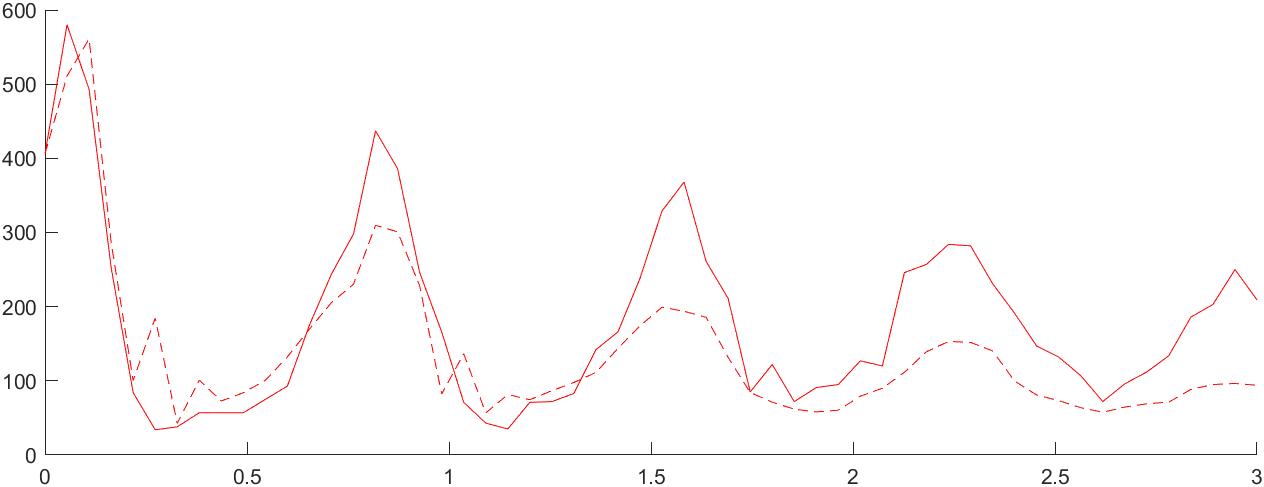
\includegraphics[height=4cm]{zad1X.png}
        \caption{Rozmiar populacji ofiar w zależności od czasu. Linią ciągłą przedstawiono pomiary rzeczywiste, przerywaną estymatę.}
    \end{figure}
     
\section{Modelowanie populacji drapieżników}
    Następnie wyznaczono wartości $r_y,r_{yx}$ i $r_{yy}$ minimalizujące wskaźnik dopasowania modelu do danych, określonego wzorem
    \begin{flalign*}
        &\quad J_y\equiv\sum\limits^{N}_{n=2}(\hat{y}_n-\tilde{y}_n)^2, &
    \end{flalign*}
    gdzie $\hat{y}_n$ ($n=2,\dots,N$) oznacza estymatę wartości $y(t_n)$, uzyskaną poprzez rozwiązanie równania (2) po podstawieniu $x(t_1)=\tilde{x}_1,\dots,x(t_N)=\tilde(x)_N$ oraz $y(t_1)=\tilde{y}_1$. Najdokładniejsze przybliżenie zostało otrzymane przy użyciu metody Adamsa-Bashfortha. Parametrami opisującymi dobrany model są 
    $r_y$=$-12.79$, $r_{yx}$=$0.07$, $r_{yy}$=$0.02$.

    \begin{figure}[h!]
        \centering
        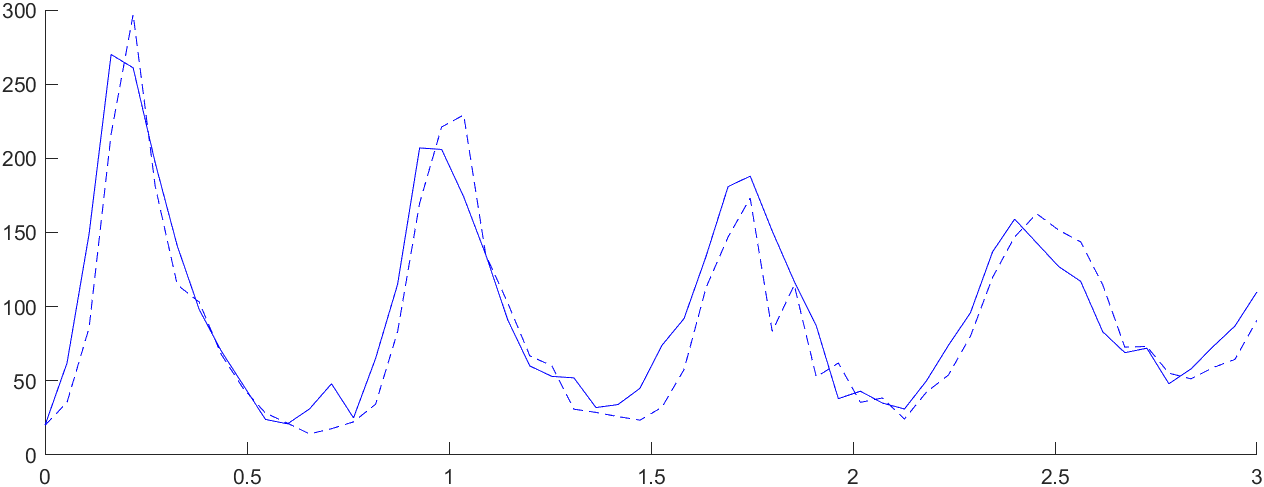
\includegraphics[height=4cm]{zad1Y.png}
        \caption{Rozmiar populacji drapieżników w zależności od czasu. Linią ciągłą przedstawiono pomiary rzeczywiste, przerywaną estymatę.}
    \end{figure}

\break

\section{Dopasowanie modelu}
    Poprzednio wyznaczone wartości parametry posłużyły do dopasowania modelu, minimalizującego wskaźnik dopasowania, określony wzorem
    \begin{flalign*}
        &\quad J\equiv\sum\limits^{N}_{n=2}(\hat{x}_n-\tilde{x}_n)^2+\sum\limits^{N}_{n=2}(\hat{y}_n-\tilde{y}_n)^2, &
    \end{flalign*}
    gdzie $\hat{x}_n,\hat{y}_n(n=2,\dots N)$ oznaczają estymat wartości $x(t_n), y(t_n),$ uzyskane poprzez rozwiązanie równań (1), (2) dla warunków początkowych $x(t_1)=\tilde{x}_1,y(t_1)=\tilde{y}_1$. Jako wartości początkowe zostały użyte wartości wyznaczone przy pomocy metody Eulera, ponieważ zapewniały one dokładniejszy wynik końcowy ($r_x=6.136346, r_{xy}=-0.069893, r_{xx}=0; r_y=-5.884900, r_{yx}=0.059108, r_{yy}=-0.033141 $).
    Do wyznaczenia wartości parametrów została użyta funkcja \textit{\textbf{fminsearch}}, a do rozwiązywania układu równań funkcja \textit{\textbf{ode45}}. Następujące parametry określają najlepszy
    model: 
    \begin{table}[h!]
    \centering
        \begin{tabular}{|l|l|l|l|l|l|}
        \hline
        $r_x$   & $r_{xy}$& $r_{xx}$ & $r_y$  & $r_{yx}$  & $r_{yy}$ \\ \hline
        $9.2205$ &  $-0.0977$ &  $0.0001$ &   $-8.1276$  &  $0.0545$  & $-0.0098$ \\ \hline
        \end{tabular}
    \end{table}
    \begin{figure}[h!]
        \centering
        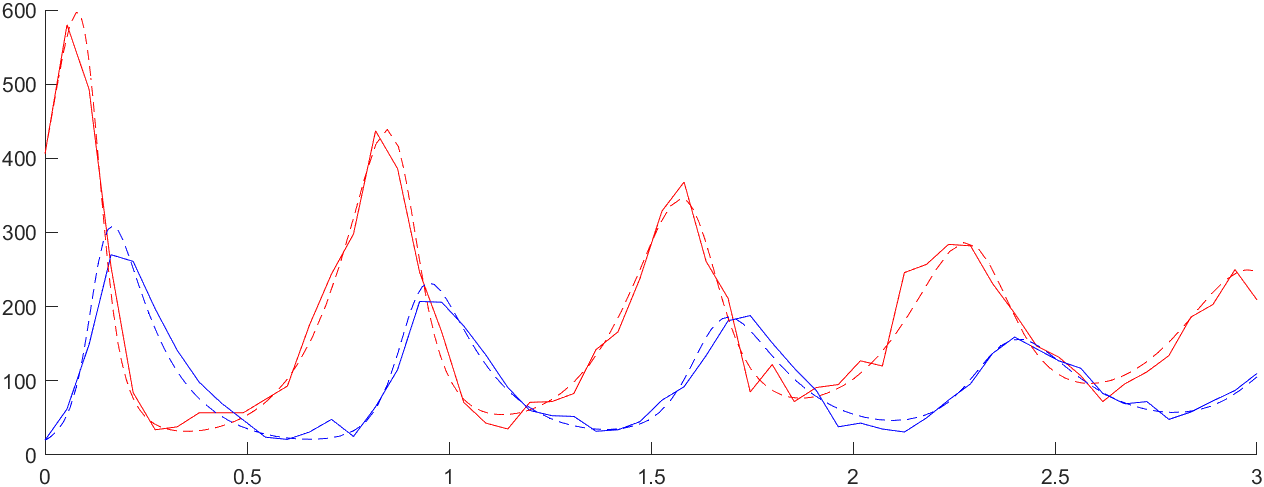
\includegraphics[height=6cm]{zad2.png}
        \caption{Rozmiar populacji drapieżników i ofiar w zależności od czas. Linią ciągłą przedstawiono pomiary rzeczywiste, przerywaną estymatę. Kolorem czerwonym oznaczono populację ofiar, niebieskim drapieżników.}
    \end{figure}

\section{Stan równowagi}
    Dla wyznaczonych wartości parametrów możliwe jest wyznaczenie wartości $x(t),y(t)$ dla których układ osiąga stan równowagi, są one rozwiązaniem układu równań (3).
    \begin{flalign}
        & \quad  0=r_xx+r_{xy}xy+r_{xx}x^2 & \notag \\
        & \quad  0=r_yy+r_{yx}xy+r_{yy}y^2 &
    \end{flalign}
    Którego rozwiązaniem jest para $x=166.1312, y=94.5457$.
\section{Modelowanie populacji Chromistów}
    Parametry $r_x$ i $r_y$ opisują naturalne tempo wzrostu populacji w optymalnych warunkach, skutkujące eksponencjalnym przyrostem.
    Uwzględnienie $r_{xx}$ oraz $r_{yy}$ pozwala wyznaczyć maksymalny rozmiar populacji, spowodowany przykładowo pełnym wykorzystaniem zasobów.
    \begin{flalign*}
        \quad \dv{x}{t}(t)=r_xx(t) \implies x(t)=x_1e^{r_xt}, 
        \quad \dv{x}{t}(t)=r_xx(t)+r_{xx}x^2(t) \implies x(t)=x_1\frac{1-r_{xx}}{r_x}\frac{r_xe^{r_xt}}{1-r_{xx}e^{r_{x}t}} &&
    \end{flalign*}
    
    Parametry $r_{xy},r_{yx}$ opisują relację międzygatunkową. Spodziewany jest negatywny wpływ drapieżników na populację ofiar ($r_{xy}<0$) oraz pozytywny ofiar na populację drapieżników ($r_{yx}>0$).\\
    
    W zadaniu zostały wykorzystane dane reprezentujące pomiary liczebności populacji chromistów \textit{Paramecium Caudatum} i \textit{Didinium Nasutum} w pewnym doświadczeniu z 1934 r. Dodatkowo wartości początkowe $\hat{x}_1$ i $\hat{y}_1$ zostały dobrane, aby minimalizować błąd estymacji. Aby zwiększyć dokładność modelowania dane zostały przeskalowane liniowo w czasie pomiędzy pomiarami. Dzięki temu możliwe było otrzymanie dokładnego modelu, określonego parametrami:
    \begin{table}[h!]
    \centering
        \begin{tabular}{|l|l|l|l|l|l|l|l|}
        \hline
        $x_1$ & $r_x$   & $r_{xy}$& $r_{xx}$ & $y_1$ & $r_y$  & $r_{yx}$  & $r_{yy}$ \\ \hline
        $1.1855$ & $20.0975$ &  $-1.2041$ &  $-0.1876$ &   $0.2924$  &  $-2.6962$  & $0.7880$ & $-0.3097$ \\ \hline
        \end{tabular}
    \end{table}
     \begin{figure}[h!]
        \centering
        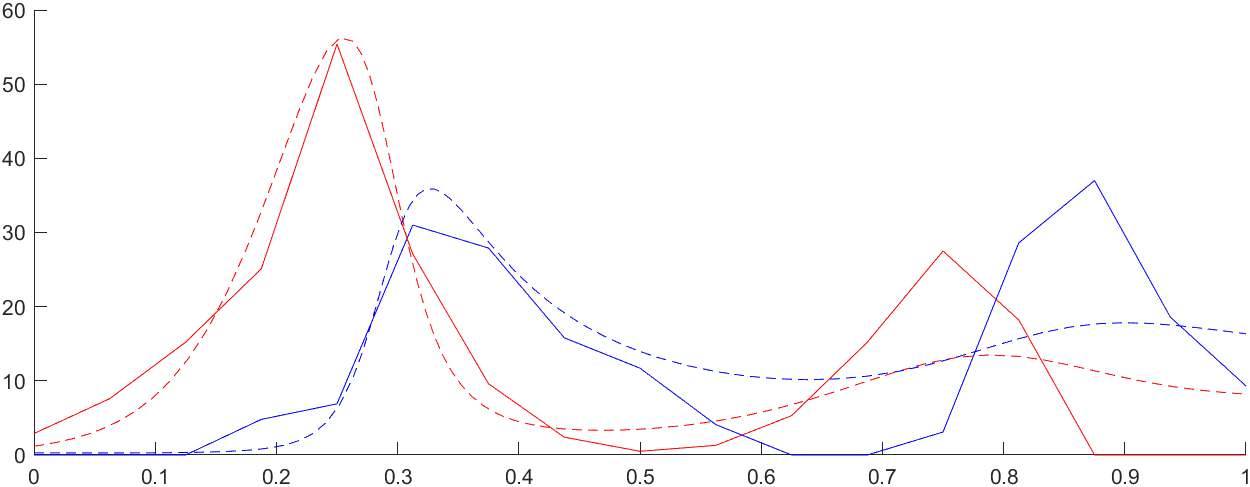
\includegraphics[height=6cm]{zad3.png}
        \caption{Rozmiar populacji drapieżników i ofiar w zależności od czas. Linią ciągłą przedstawiono pomiary rzeczywiste, przerywaną estymatę. Kolorem czerwonym oznaczono populację ofiar, niebieskim drapieżników.}
    \end{figure}   

\break
\section{Wykorzystane programy}
\tiny
\begin{lstlisting}[caption=Zadanie 1a]
data = readtable('dane21.csv');
N1 = 20; N2 = 20; N3 = 20;
J = zeros(N1,N2,N3);
RX = linspace(-100,100,N2);
RXY = linspace(-1,1,N2);
RXX = linspace(-1,1,N3);
dt = mean(diff(data.t));
T = 0 :  dt : 3;

for it1 = 1 : N1
    for it2 = 1 : N2
        for it3 = 1 : N3
            rx = RX(it1);
            rxy = RXY(it2);
            rxx = RXX(it3);
            x = zeros(size(T));
            x(1) = data.x(1);
            f = @(x,y) rx*x+rxy*x*y+rxx*x*x;
%             Metoda Eulera
%             for i = 2 : length(T)
%                 x(i) = x(i-1) + dt * f(x(i-1), data.y(i-1));
%             end

%             Adams-Bashforth
            x(2) = x(1) + dt * f(x(1), data.y(1));
            x(3) = x(2) + dt * f(x(2), data.y(2));
            for i = 4 : length(T)
                x(i) = x(i-1) + dt/12 * (23*f(x(i-1), data.y(i-1))...
                    -16*f(x(i-2), data.y(i-2)) +5*f(x(i-3), data.y(i-3)));
            end

%             Niejawna metoda Eulera
%             for i = 2 : length(T)
%                 x1 = -(dt*rx - (dt^2*rx^2 + 2*dt^2*rx*rxy*data.y(i) + dt^2*rxy^2*data.y(i)^2 - 2*dt*rx - 2*dt*rxy*data.y(i) - 4*rxx*x(i-1)*dt + 1)^(1/2) + dt*rxy*data.y(i) - 1)/(2*dt*rxx);
%                 x2 = -(dt*rx + (dt^2*rx^2 + 2*dt^2*rx*rxy*data.y(i) + dt^2*rxy^2*data.y(i)^2 - 2*dt*rx - 2*dt*rxy*data.y(i) - 4*rxx*x(i-1)*dt + 1)^(1/2) + dt*rxy*data.y(i) - 1)/(2*dt*rxx);
%                 if isreal(x1) && isreal(x2) && (x1>0 || x2>0)
%                     x(i) = max(x1, x2);
%                 else
%                     x(i) = Inf;
%                     break
%                 end
%             end

            J(it1, it2, it3) = sum((data.x'-x).*(data.x'-x));
        end
    end
end
[v, ind] = min(J(:));
[it1, it2, it3] = ind2sub(size(J), ind);
A = fminsearch(@(X) ApproxX(X(1), X(2), X(3)), [RX(it1), RXY(it2), RXX(it3)]);
fprintf("r_x=%f; r_xy=%f; r_xx=%f;\n", A(1), A(2), A(3));

function [J] = ApproxX(rx ,rxy, rxx)
data = readtable('dane21.csv');
dt = mean(diff(data.t));
T = 0 :  dt : 3;
x = zeros(1, length(T));
x(1) = data.x(1);

for i = 2 : length(T)
    x1 = -(dt*rx - (dt^2*rx^2 + 2*dt^2*rx*rxy*data.y(i) + dt^2*rxy^2*data.y(i)^2 - 2*dt*rx - 2*dt*rxy*data.y(i) - 4*rxx*x(i-1)*dt + 1)^(1/2) + dt*rxy*data.y(i) - 1)/(2*dt*rxx);
    x2 = -(dt*rx + (dt^2*rx^2 + 2*dt^2*rx*rxy*data.y(i) + dt^2*rxy^2*data.y(i)^2 - 2*dt*rx - 2*dt*rxy*data.y(i) - 4*rxx*x(i-1)*dt + 1)^(1/2) + dt*rxy*data.y(i) - 1)/(2*dt*rxx);
    if isreal(x1) && isreal(x2) && (x1>0 || x2>0)
        x(i) = max(x1, x2);
    else
        x(i) = Inf;
        break
    end
end
J = sum((data.x'-x(1,:)).*(data.x'-x(1, :)));
end % function
\end{lstlisting}

\break

\begin{lstlisting}[caption=Zadanie 1b]
data = readtable('dane21.csv');
N1 = 50;
N2 = 50;
N3 = 50;
J = zeros(N1,N2,N3);
RY = linspace(-100,100,N1);
RYX = linspace(-1,1,N2);
RYY = linspace(-1,1,N3);
dt = mean(diff(data.t));
T = 0 :  dt : 3;
for it1 = 1 : N1
    for it2 = 1 : N2
        for it3 = 1 : N3
            ry = RY(it1);
            ryx = RYX(it2);
            ryy = RYY(it3);
            y = zeros(size(T));
            y(1) = data.y(1);
            f = @(x,y) ry*y+ryx*x*y+ryy*y*y;
%             Metoda Eulera
%             for i = 2 : length(T)
%                 y(i) = y(i-1) + dt*f(data.x(i-1), y(i-1));
%             end

%             Metoda Adamsa-Bashfortha
            y(2) = y(1) + dt * f(data.x(1), y(1));
            y(3) = y(2) + dt * f(data.x(2), y(2));
            for i = 4 : length(T)
                y(i) = y(i-1) + dt/12 * (23*f(data.x(i-1), y(i-1))...
                    -16*f(data.x(i-2), y(i-2)) +5*f(data.x(i-3), y(i-3)));
            end

%             Niejawna metoda Eulera
%             for i = 2 : length(T)
%                 y1 = -(dt*ry - (dt^2*ry^2 + 2*dt^2*ry*ryx*data.x(i) + dt^2*ryx^2*data.x(i)^2 - 2*dt*ry - 2*dt*ryx*data.x(i) - 4*ryy*y(i-1)*dt + 1)^(1/2) + dt*ryx*data.x(i) - 1)/(2*dt*ryy);
%                 y2 = -(dt*ry + (dt^2*ry^2 + 2*dt^2*ry*ryx*data.x(i) + dt^2*ryx^2*data.x(i)^2 - 2*dt*ry - 2*dt*ryx*data.x(i) - 4*ryy*y(i-1)*dt + 1)^(1/2) + dt*ryx*data.x(i) - 1)/(2*dt*ryy);
%                 if isreal(y1) && isreal(y2) && (y1>0 || y2>0)
%                     y(i) = max(y1, y2);
%                 else
%                     y(i) = Inf;
%                     break
%                 end
%             end

            J(it1, it2, it3) = sum((data.y'-y).*(data.y'-y));
        end
    end
end

[v, ind] = min(J(:));
[it1, it2, it3] = ind2sub(size(J), ind);
A = fminsearch(@(X) ApproxY(X(1), X(2), X(3)), [RY(it1), RYX(it2), RYY(it3)]);
fprintf("r_y=%f; r_yx=%f; r_yy=%f;\n", A(1), A(2), A(3));

function [J] = ApproxY(ry, ryx, ryy)
data = readtable('dane21.csv');
dt = mean(diff(data.t));
T = 0 :  dt : 3;
y = zeros(size(T));
y(1) = data.y(1);
for i = 2 : length(T)
    y1 = -(dt*ry - (dt^2*ry^2 + 2*dt^2*ry*ryx*data.x(i) + dt^2*ryx^2*data.x(i)^2 - 2*dt*ry - 2*dt*ryx*data.x(i) - 4*ryy*y(i-1)*dt + 1)^(1/2) + dt*ryx*data.x(i) - 1)/(2*dt*ryy);
    y2 = -(dt*ry + (dt^2*ry^2 + 2*dt^2*ry*ryx*data.x(i) + dt^2*ryx^2*data.x(i)^2 - 2*dt*ry - 2*dt*ryx*data.x(i) - 4*ryy*y(i-1)*dt + 1)^(1/2) + dt*ryx*data.x(i) - 1)/(2*dt*ryy);
    if isreal(y1) && isreal(y2) && (y1>0 || y2>0)
        y(i) = max(y1, y2);
    else
        y(i) = Inf;
        break
    end
end
J= sum((data.y'-y).*(data.y'-y));
end % function
\end{lstlisting}

\break

\begin{lstlisting}[caption=Zadanie 2]
data = readtable('dane21.csv');
J = @(X) fun(X(1), X(2),X(3),X(4),X(5),X(6));

r_x=6.136346; r_xy=-0.069893; r_xx=-0.000000;
r_y=-5.884900; r_yx=0.059108; r_yy=-0.033141;

[W, val] = fminsearch(J, [r_x, r_y, r_xy, r_yx, r_xx, r_yy]);
disp(W);

f = figure;
hold on 
f.Position = [100 100 1000 350];
plot(data.t, data.x,'r');
plot(data.t, data.y,'b');
f = @(t,x) [W(1)*x(1) + W(3)*x(1)*x(2)+ W(5)*x(1)*x(1); ...
    W(2)*x(2) + W(4)*x(1)*x(2) + W(6)*x(2)*x(2)];
[t,y] = ode45(f, [0 3], [data.x(1), data.y(1)]);
plot(t,y(:,1),'r--');
plot(t,y(:,2),'b--');

function J = fun(rx, ry, rxy, ryx, rxx, ryy)
    data = readtable('dane21.csv');
    
    f = @(t, x) [rx*x(1) + rxy*x(1)*x(2)+rxx*x(1)*x(1); ...
        ry*x(2) + ryx*x(1)*x(2) + ryy*x(2)*x(2)];

    [t, y] = ode45(f, [0 3], [data.x(1), data.y(1)]);
    X = interp1(t, y, data.t);
    J = sum( (X-[data.x, data.y]).*(X-[data.x, data.y]), 'all'); 
end % function
\end{lstlisting}

\begin{lstlisting}[caption=Zadanie 3]
data = readtable('Chromista.csv');
data = renamevars(data, data.Properties.VariableNames, ["t", "x", "y"]);
data.t = normalize(data.t, 'range');
SCALING = 5;

N1 = 20; N2 = 20; N3 = 20; N4 = 20;
J = zeros(N1,N2,N3, N4);
RX = linspace(0,50,N1);
RXY = linspace(-3,0,N2);
RXX = linspace(-1,1,N3);
X = linspace(min(data.x),max(data.x),N4);
dt = mean(diff(data.t))/SCALING;
T = 0 : dt : 1;
YInterp = interp1(data.t, data.y, T);
XInterp = interp1(data.t, data.x, T);

for it1 = 1 : N1
    for it2 = 1 : N2
        for it3 = 1 : N3
            for it4 = 1 : N4
                rx = RX(it1);
                rxy = RXY(it2);
                rxx = RXX(it3);
                x = zeros(size(T));
                x(1) = X(it4);
                f = @(x,y) rx*x+rxy*x*y+rxx*x*x;
                x(2) = x(1) + dt * f(x(1), YInterp(1));
                x(3) = x(2) + dt * f(x(2), YInterp(2));
                for i = 4 : length(T)
                    x(i) = x(i-1) + dt/12 * (23*f(x(i-1), YInterp(i-1))...
                        -16*f(x(i-2), YInterp(i-2)) +5*f(x(i-3), YInterp(i-3)));
                end
                J(it1, it2, it3, it4) = sum((XInterp-x).*(XInterp-x));
            end
        end
    end
end
[~, ind] = min(J(:));
[it1, it2, it3, it4] = ind2sub(size(J), ind);
A = fminsearch(@(X) ApproxX(X(1), X(2), X(3), X(4)), [RX(it1), RXY(it2), RXX(it3), X(it4)], optimset('Display','off'));
r_x=A(1); r_xy=A(2); r_xx=A(3); x0=A(4);

J = zeros(N1,N2,N3, N4);
RY = linspace(-30,0,N1);
RYX = linspace(0,3,N2);
RYY = linspace(-1,1,N3);
Y = linspace(min(data.y),max(data.y),N4);
for it1 = 1 : N1
    for it2 = 1 : N2
        for it3 = 1 : N3
            for it4 = 1 : N4
                ry = RY(it1);
                ryx = RYX(it2);
                ryy = RYY(it3);
                y = zeros(size(T));
                y(1) = Y(it4);
                f = @(x,y) ry*y+ryx*x*y+ryy*y*y;
                y(2) = y(1) + dt * f(data.x(1), y(1));
                y(3) = y(2) + dt * f(data.x(2), y(2));
                for i = 4 : length(T)
                    y(i) = y(i-1) + dt/12 * (23*f(XInterp(i-1), y(i-1))...
                        -16*f(XInterp(i-2), y(i-2)) +5*f(XInterp(i-3), y(i-3)));
                end
                J(it1, it2, it3, it4) = sum((YInterp-y).*(YInterp-y));
            end
        end
    end
end
[v, ind] = min(J(:));
[it1, it2, it3, it4] = ind2sub(size(J), ind);
A = fminsearch(@(X) ApproxY(X(1), X(2), X(3), X(4)), [RY(it1), RYX(it2), RYY(it3), Y(it4)], optimset('Display','off'));
r_y=A(1); r_yx=A(2); r_yy=A(3); y0=A(4);

J = @(X) fun3(X(1), X(2), X(3), X(4), X(5), X(6), X(7), X(8));
W = fminsearch(J, [x0, y0, r_x, r_y, r_xy, r_yx, r_xx, r_yy], optimset('Display','off'));
disp(W)

f=figure;
hold on
f.Position = [100 100 1000 350];
plot(data.t, data.x,'r');
plot(data.t, data.y,'b');
f = @(t,x) [W(3)*x(1) + W(5)*x(1)*x(2)+ W(7)*x(1)*x(1); ...
    W(4)*x(2) + W(6)*x(1)*x(2) + W(8)*x(2)*x(2)];
[t,y] = ode45(f, [0 1], [W(1), W(2)]);
plot(t,y(:,1),'r--');
plot(t,y(:,2),'b--');

function [J] = ApproxX(rx ,rxy, rxx, x0)
data = readtable('Chromista.csv');
data = renamevars(data, data.Properties.VariableNames, ["t", "x", "y"]);
SCALING = 5;
dt = mean(diff(data.t))/SCALING;
T = 0:dt:1;
YInterp = interp1(data.t, data.y, T);
XInterp = interp1(data.t, data.x, T);
data.t = normalize(data.t, 'range');

x = zeros(1, length(T));
x(1) = x0;
f = @(x,y) rx*x+rxy*x*y+rxx*x*x;
x(2) = x(1) + dt * f(x(1), YInterp(1));
x(3) = x(2) + dt * f(x(2), YInterp(2));
for i = 4 : length(T)
    x(i) = x(i-1) + dt/12 * (23*f(x(i-1), YInterp(i-1))...
        -16*f(x(i-2), YInterp(i-2)) +5*f(x(i-3), YInterp(i-3)));
end
J = sum((XInterp-x).*(XInterp-x));
end % function

function [J] = ApproxY(ry, ryx, ryy, y0)
data = readtable('Chromista.csv');
data = renamevars(data, data.Properties.VariableNames, ["t", "x", "y"]);
SCALING = 5;
dt = mean(diff(data.t))/SCALING;
T = 0:dt:1;
YInterp = interp1(data.t, data.y, T);
XInterp = interp1(data.t, data.x, T);
data.t = normalize(data.t, 'range');
dt = mean(diff(data.t));
y = zeros(1, length(T));
y(1) = y0;
f = @(x,y) ry*y+ryx*x*y+ryy*y*y;
y(2) = y(1) + dt * f(data.x(1), y(1));
y(3) = y(2) + dt * f(data.x(2), y(2));
for i = 4 : length(T)
    y(i) = y(i-1) + dt/12 * (23*f(XInterp(i-1), y(i-1))...
        -16*f(XInterp(i-2), y(i-2)) +5*f(XInterp(i-3), y(i-3)));
end
J= sum((YInterp-y).*(YInterp-y));
end % function

function J = fun3(x1, y1, rx, ry, rxy, ryx, rxx, ryy)
data = readtable('Chromista.csv');
data = renamevars(data, data.Properties.VariableNames, ["t", "x", "y"]);
data.t = normalize(data.t, 'range');
f = @(t, x) [rx*x(1) + rxy*x(1)*x(2)+rxx*x(1)*x(1); ...
    ry*x(2) + ryx*x(1)*x(2) + ryy*x(2)*x(2)];
[t, y] = ode45(f, [0 1], [x1, y1]);
X = interp1(t, y, data.t);
J = sum( (X-[data.x, data.y]).*(X-[data.x, data.y]), 'all');
end % function
\end{lstlisting}
\end{document}